% Two distinct methods exist for THz generation and detection using ultrafast quantum cascade laser systems. THz radiation can be generated or detected by making use of non-linear optics. Non-linear optics exploit crystals with large second-order non-linear susceptibilities \cite{THzSourcesDetectors, kimHighlyNonlinearOptical2021} for THz generation or detection. By using a photoconductive material and utilizing the concept of photomixing, THz waves can also be generated or detected. This thesis will only focus on the photoconductive approach. 

PCAs are among the most established devices for generating and detecting THz radiation. They operate as ultrafast optical switches. When a laser pulse illuminates the photoconductor, its conductivity increases abruptly due to the generation of electron-hole pairs. A bias voltage applied across the electrodes accelerates these carriers, producing a photocurrent that drives THz radiation in the antenna structure.  

Efficient THz emission requires sub-picosecond switching. The switch-on time is governed by the excitation laser pulse duration, while the switch-off time is limited by the carrier lifetime of the semiconductor material. Suitable PCA substrates must therefore combine short carrier lifetimes with high carrier mobility and high breakdown voltage to ensure both ultrafast response and robust operation.  

A PCA consists of a small active photoconductive region between metallic electrodes. The electrodes provide the bias field and couple the transient photocurrent into free-space radiation. The underlying physical mechanisms and corresponding mathematical description are discussed in the following sections.



% PCAs are one of the most established for generating and detecting THz radiation. A PCA is a semiconductor device that acts as an optical switch by increasing its conductivity when illuminated. The semiconductor device (photoconductor) features a direct band-gap. Photoconductors are operated with lasers and are based on the principle of photomixing \cite{peytavitTHzPhotomixers2021}. Two interfering laser beams forming an optical beat signal are focused on the photoconductor. When the beat signal's energy level is higher than that of the semiconductor's band-gap energy, free electron-hole pairs are photo-generated. A bias voltage applied to the electrodes of the antenna separates the carriers to create a displacement current. The current oscillates with the envelope of the absorbed laser light, resulting in a THz signal \cite{nandiErAsInAlGaAsPhotoconductors2021}. To emit or detect THz radiation, the switching in a PCA must happen within a subpicosecond timescale. The switch-on time depends on the duration of the laser pulse. The switch-off time is mainly determined by the lifetime of photoexcited carriers in the semiconductor. Both a short laser pulse and a short carrier lifetime are essential for ultrafast switching. High carrier mobility and high breakdown voltage are also important for achieving good material performance. PCAs usually consist of a photomixing device, often called active region, sitting in between the antenna's electrodes. The electrodes help emit or detect the THz signal. The mathematics for THz generation through photomixing are given in the following sections. 

\subsection{Principles of Photomixing for Pulsed Operation}
To explain the principles of pulsed operation for THz-TDS, continuos wave (CW) operation (see Figure \ref{fig:cw_basics}) is explained beforehand. The principles of pulsed operation are then derived from CW operation. This section is mainly a review of \cite{nandiErAsInAlGaAsPhotoconductors2021,faridiPulsedFreeSpace2023,preuPrinciplesTHzGeneration2015}.

\begin{figure}
	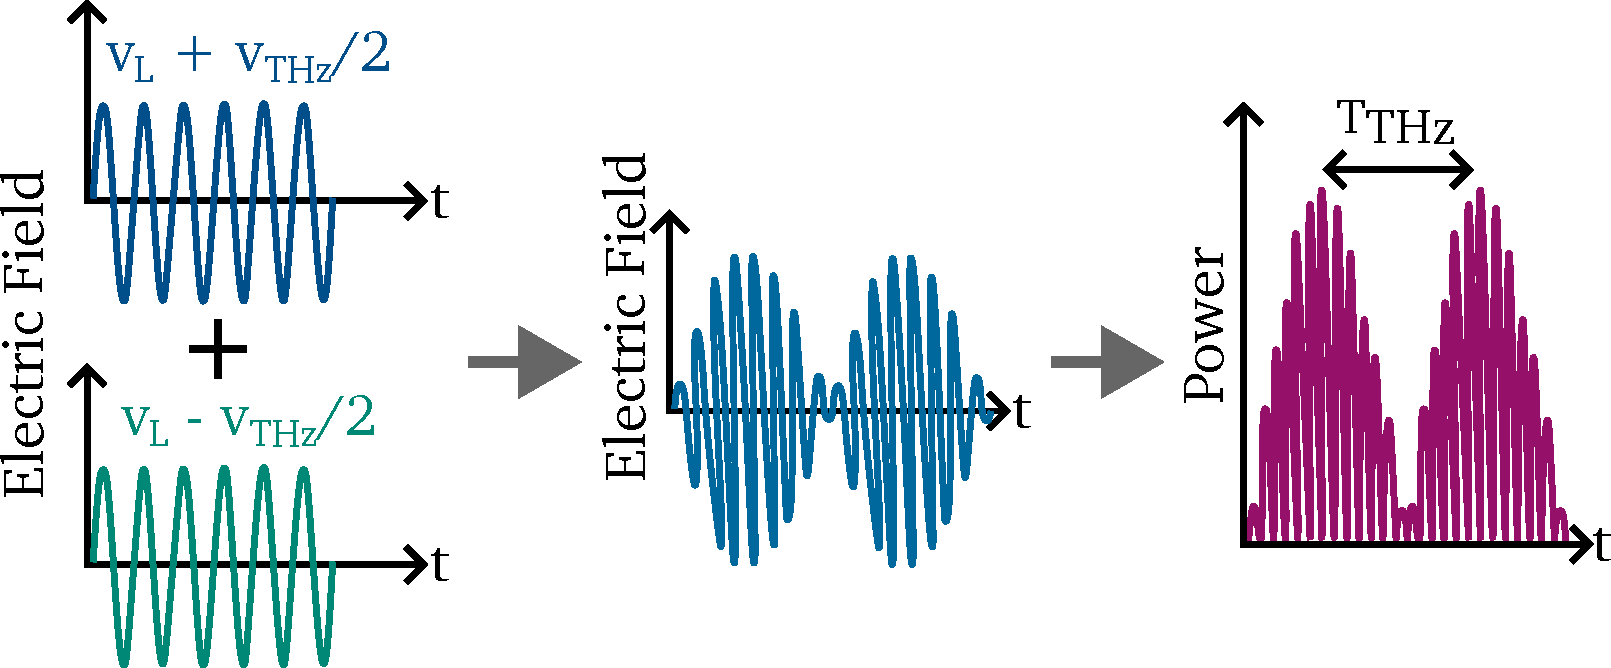
\includegraphics[width=0.85\linewidth]{figures/cw_principles.pdf}
	\centering
	\caption{Basic working principle of the continuos wave photomixing process. Two laser signals are heterodyned. The resulting power modulation shows a beat node at the difference frequency $\nu_{THz} = 1/T_{THz}$ of the two signals.}
	\label{fig:cw_basics}
\end{figure}

\subsubsection{CW operation}
In CW photomixing, two single-mode lasers operate at a difference frequency $\omega_L = \omega_0 \pm \omega_{THz}$. The two laser signals are heterodyned, producing an intensity beat at the difference frequency of the two lasers. The photoconductor is illuminated by the heterodyned laser signal. If the modulation of the lasers exceeds the semiconductor band-gap energy, charge carriers are generated at the beat frequency. The heterodyned signal illuminating the photoconductor is given by 
% CW THz radiation is generated using two CW lasers. The lasers have a difference frequency of $\omega_L = \omega_0 \pm \omega_{THz}$. The photon energy of the lasers has to be higher than the band-gap energy of the photoconducting material: $h\nu_L > E_G$, 
% where $\nu_L = \omega_L / 2\pi$, $h$ is Planck’s constant and $E_G$ is the bandgap energy of the material. The two laser signals are heterodyned. Heterodyning means mixing two signal's frequencies to achieve a resulting signal frequency that is shifted into another frequency range. A fiber coupler is used for feeding the heterodyned signal into the photoconductor with an optical field of

\begin{equation}
	\vec{E}(t) = \vec{E}_1(t) + \vec{E}_2(t) = \vec{E}_{1,0}e^{i(\omega_L - \omega_{THz}/2)t} + \vec{E}_{2,0}e^{i(\omega_L + \omega_{THz}/2)t - i\phi},
\end{equation}
where $\phi$ is the phase difference of the laser signals. The optical intensity of the absorbed laser power is given by 
\begin{equation}
	I_L(t) \sim |\vec{E}(t)|^2 = |\vec{E}_{1,0}(t)|^2 + |\vec{E}_{2,0}(t)|^2 + 2|\vec{E}_{1,0}(t) \cdot \vec{E}_{2,0}(t)|\cos(\omega_{THz}t + \phi), 
\end{equation}

which can be rewritten in terms of laser power as 

\begin{equation}
	P_L(t) = P_1 + P_2 + 2\sqrt{P_1 P_2}\cos(\beta)\cos(\omega_{THz}t + \phi), 
\end{equation}

where $\beta$ is the angle between the polarization of the electric fields. In an ideal photoconductor, all laser light is absorbed. This yields an ideal photocurrent 
\begin{equation}
	I_{Ph}^{Id}(t) = \frac{eP_L(t)}{h\nu_L} = \frac{e(P_1+P_2)}{h\nu_L} + 2\frac{e\sqrt{P_1P_2}}{h\nu_L}\cos(\beta)\cdot\cos(\omega_{THz}t + \phi),
	\label{eq_iph}
\end{equation}

where $e$ denotes the elementary charge.
We see that the ideal photocurrent $I_{Ph}^{Id}(t)$ consists of a DC component $I_{DC}^{Id}$ and an AC component $I_{THz}^{Id}(t)$.
The DC component is given by 
\begin{equation}
	I_{DC}^{Id} = \frac{e(P_1+P_2)}{h\nu_L}.
\end{equation} 
The AC component of the ideal photocurrent is given by the expression
\begin{equation}
	I_{THz}^{Id}(t) = 2\frac{e\sqrt{P_1P_2}}{h\nu_L}\cos(\beta)\cdot\cos(\omega_{THz}t + \phi).
\end{equation}

To maximize the THz output, the AC part of the photocurrent has to be maximized. We see that $I_{THz}^{Id}$ is at its maximum when $P_1 = P_2 = P_L = P_{tot} / 2$ and $\beta = 0$. This is equivalent to identical power and polarization of the two laser signals. With these assumptions the amplitude of the ideal photocurrent's THz part becomes $I_{THz}^{Id} = eP_{tot} / (h\nu) = I_{DC}^{Id} = I^{Id}$. Ultimately inserting our assumptions into \ref{eq_iph} we get 
\begin{equation}
	I_{Ph}^{Id} = I^{Id}[1 + \cos(\omega_{THz}t + \phi)].
	\label{eq8}
\end{equation}

The generated photocurrent is fed into a radiating element, usually an antenna. This antenna is fabricated on the same semiconducting material as the photomixing device. The antenna shows a radiation resistance $R_A$, yielding the ideal emitted THz power 
\begin{equation}
	P_{THz}^{Id}=\frac{1}{2}R_A (I_{THz}^{Id})^2.
	\label{eq_thz_pow}
\end{equation}

\subsubsection{Pulsed Operation}

In pulsed operation, the semiconductor absorbs a short optical pulse. The photocurrent generated by this pulse results in THz radiation when fed into a radiating element like an antenna. The emitted THz field is proportional to the time derivative of the photocurrent generated by the lasers \cite{preuTunableContinuouswaveTerahertz2011}
\begin{equation}
	E_{THz} \propto \frac{\partial I_{Ph}(t)}{\partial t}.
\label{eq1}
\end{equation}

The CW generation of THz radiation can be extended to the pulsed approach. Under pulsed operation, multiple laser frequencies are mixed to form a single laser pulse denoted by 
\begin{equation}
	\vec{E}(t) = \sum_j^n \vec{E}_je^{i(\omega_j t + \phi j)}.
\label{eq3}
\end{equation}
Here, $\omega_j = 2 \pi \nu_j$ are the angular frequency components of each electrical field $\vec{E}_j$ and $\phi_j$ are the corresponding phase components. Assuming a typical mode locked femtosecond laser we get the following properties: 
\renewcommand{\labelenumi}{\alph{enumi})}
\begin{enumerate}
	\item The frequency components are equally spaced in the spectral domain: $\nu_j - \nu_{j-1} = R_p$, where $R_p$ is the repetition rate of the laser.
	\item The phase has a fixed, linear relationship: $\phi_j - \phi_{j-1} = const.$
\end{enumerate}

The mode locking allows for very short laser pulses in the femtosecond range.

To obtain the ideal frequency spectrum of the emitted THz field, the signal has to be Fourier transformed. Fourier transforming eq. \eqref{eq1} yields

\begin{equation}
	E_{THz}(\omega) \propto \mathcal{F}\left\{ \frac{\partial I_{Ph}(t)}{\partial t} \right\} = i\omega I_{Ph}(t), 
\end{equation}

where $\mathcal{F}\{\cdot \}$ denotes the Fourier transform and $I_{Ph}(\omega)$ is the spectrum of the photocurrent. Ideally, the spectrum of the photocurrent is proportional to the spectral width of the photocurrent. Note that the spectral width $\Delta \omega$ is inversely proportional to the temporal width $\Delta \tau$, resulting in $\Delta \omega \Delta \tau = 0.5$ The optical pulse duration must be shorter than the period of the maximum THz frequency to be obtained. 

Deriving the emitted THz spectrum under pulsed operation is fairly complex and would be beyond the scope of this thesis. Detailed derivations can be found in \cite{preuPrinciplesTHzGeneration2015}. In the following, only some fundamental steps in obtaining the emitted THz field are given. From eq. \eqref{eq1} we know that the field generated by a radiating structure like an antenna is proportional to the time-derivative of the current. We also know that the ideal photocurrent is proportional to the total optical power. Assuming a laser beam that shows Gaussian distributed intensity, meaning $\vec{E}_j$ is Gaussian distributed, eq. \eqref{eq3} becomes
\begin{equation}
	\vec{E}(t) = \vec{A}(t)e^{i\omega_Lt}.
\label{eq4} 
\end{equation}

$\vec{A}(t)$ denotes the complex envelope of the pulse while $\omega_L$ is the laser pulses central frequency. With the mode-locked laser property of a linear phase relationship, the pulse is Fourier transform-limited (bandwidth-limited), yielding an envelope of
\begin{equation}
	\vec{A}(t) = \vec{A}_0 e^{\frac{-t^2}{\tau^2}},
\end{equation}

with $\tau$ being the time-domain $1/e^2$ width. The  $1/e^2$ width is the difference of the two points in the Gaussian beam where the intensity falls to $1/e^2 = 0.135$. 

The Gaussian pulse's optical intensity is once again given by
\begin{equation}
	I_L(t) \sim |\vec{E}_L(t)|^2 = I_{L,0}e^{\frac{-2t^2}{\tau ^2}}.
\end{equation} 

Note that $I_{L,0} \sim |\vec{A}_0|^2$ which corresponds to the peak intensity of the beam. 
Fourier transforming eq. \eqref{eq4} gives us the spectral components of the pulse:

\begin{equation}
	V(\nu) =  \mathcal{F}\left\{\vec{A}(t)e^{i\omega_Lt} \right\}
	= \int_{-\infty}^{+\infty}E_L(t)e^{-i2\pi\nu t}dt = |V(\nu)|e^{i\psi(\nu)}.
\end{equation}

$\psi(\nu)$ denotes the spectral phase in this case. For a Gaussian beam, the spectral intensity is given by:
\begin{equation}
	S_I(\nu) = |V(\nu)|^2 \sim \exp[-2\pi^2\tau^2(\nu - \nu_L)^2]. 
\end{equation}

The spectral $1/e^2$ width here is described by $\sigma$, with $\tau = \sqrt{2}/(\pi \sigma)$. We already know from eq. \eqref{eq_iph} that the photocurrent is proportional to the laser power, $I_{Ph}(t) \sim P_L(t)$. Thus the ideal generated photocurrent can be expressed as 

\begin{equation}
	I_{Ph}^{Id}(t) = \frac{eP_L(t)}{h\nu_L} = \hat{I}_{L,0} e^{\frac{-2t^2}{\tau^2}},
\label{eq_gauss}
\end{equation}

where $\hat{I}_{L,0}$ is the maximum generated photocurrent. From eq. \eqref{eq_gauss} we can conclude that in an ideal case, the resulting photocurrent is Gaussian distributed because the carriers respond to the lasers envelope. 

\subsection{Principles of THz Detection by Photomixing for Pulsed Operation}

Photoconductors can also act as THz detectors, based on the same mechanisms as generation. Implementing PCA based THz detectors is explained in the following as a review of \cite{preuPrinciplesTHzGeneration2015,castro-camusPhotoconductiveResponseCorrection2008}. An ultrafast laser pulse and a THz transient are focused onto the active region between the antenna electrodes. The laser pulse generates electron–hole pairs. The incident THz field provides the bias, modulating charge-carrier motion. Since both signals overlap in space and time, the photocurrent is given by the convolution of the optical pulse with the THz field. The photocurrent is heavily dependent on the incident THz field and the conductivity of the semiconducting material. The latter defines the mode of operation in THz detection. Photoconductive detectors work in direct sampling or integrating mode. They can also be configured to be used in intermediate sampling modes, depending on the semiconducting properties.

% An ultrafast laser pulse and a THz signal generated by the same laser signal are focused onto the active region in between the antenna electrodes. The optical pulse of the laser creates free electron-hole pairs that can be converted into a current by applying a bias field. This bias field is provided by the incoming THz signal. The electrical field of the THz signal controls the current flow. As the laser signal and the incoming THz signal incite the active region simultaneously, the photocurrent is given by convolution of the two signals. The generated DC current is heavily dependent on the incoming THz field and the conductivity of the semiconducting material. The latter defines the mode of operation in THz detection. Photoconductive detectors work in direct sampling or integrating mode. They can also be configured to be used in intermediate sampling modes, depending on the semiconducting properties.

\subsubsection{Direct Sampling}

In materials with ultrashort carrier lifetimes ($\tau_c \ll 1$\,\si{\pico \s}), charge-carriers recombine almost immediately. This produces a delta-like conductivity spike, only lasting as long as the device is illuminated. The photocurrent thus samples the instantaneous THz field:
\begin{equation}
    I(\tau) \propto E_{THz}(t=\tau).
\end{equation}
By varying the temporal overlap $\tau$ between laser and THz pulse, the transient field can be reconstructed.

% Direct sampling detectors work by exploiting the properties of highly resistive semiconducting materials which exhibit very low charge-carrier lifetimes $\tau_c \ll 1$ \si{\pico \s}. The optically generated charge-carriers are trapped very quickly by scattering and trapping centers in the semiconductor's crystal structure. The generated electron-hole pairs provide a conductivity spike which only lasts as long as the device is illuminated by the laser pulse. In an ideal case, the conductivity spike can be modeled as a delta function. As the generated photocurrent is given by the convolution of the laser pulse and the incoming THz radiation, in this case, it only samples the point of the THz signal that overlaps spatially and temporally with the laser pulse. This means that the incoming THz transient can be reconstructed by changing the temporal overlap $\tau$ between the laser pulse and the THz wave. Assuming the spike in conductivity to be much shorter than the THz signal's transient features, the THz wave is given by

% \begin{equation}
% 	I(\tau) \propto E_{THz}(t=\tau).
% \end{equation}

\subsubsection{Integrating Detection}
For long carrier lifetimes ($\tau_c > 1$\,\si{\pico \s}), the photoconductor remains conductive well beyond the duration of the THz transient. The photocurrent is given by the integral over the convolution of the transient electrical field and the material conductivity $\sigma(t)$:
\begin{equation}
    I(\tau) \propto \int_{-\infty}^{+\infty} E_{THz}(t)\sigma(t=\tau)\, dt .
    \label{eq_conv_integration_detection}
\end{equation}
Assuming a step-like conductivity, this reduces to
\begin{equation}
    I(\tau) \propto \int_{\tau}^{+\infty} E_{THz}(t)\, dt.
    \label{eq_conv_int_det_2}
\end{equation}
The THz field can be reconstructed by differentiating the detected photocurrent with respect to time. Long-lifetime devices enable high bandwidth (limited by the laser pulse duration) but also integrate noise, ultimately lowering SNR. In practice, optimal detection combines aspects of direct and integrating operation.

\subsubsection{Intermediate Case and Deconvolution}

For carrier lifetimes comparable to the THz pulse duration, the photocurrent cannot be directly related to $E_{THz}(t)$ by proportionality or differentiation. Instead, a convolution approach is used \cite{castro-camusPhotoconductiveResponseCorrection2008}:
\begin{equation}
    I(\tau) \propto \beta \int_{-\infty}^{+\infty} E_{THz}(t)\Phi(t-\tau)\, dt ,
    \qquad \beta \propto P_L T_{12} \lambda ,
    \label{eq_conv_integration_detection_2}
\end{equation}
with $\Phi(t) = \theta(t)e^{-t/\tau_{rec}}$ the normalized conductivity response and $T_{12}$ the Fresnel transformation coefficient. Fourier transforming yields
\begin{equation}
    I(\omega) = \beta E_{THz}(\omega)\Phi(\omega).
    \label{eq_FFT_int_det}
\end{equation}
The THz field follows by inverse transform:
\begin{equation}
    E_{THz}(t) = \frac{1}{\beta} \mathcal{F}^{-1}\left\{\frac{I(\omega)}{\Phi(\omega)}\right\}
    = \frac{1}{\beta} \mathcal{F}^{-1}\left\{I(\omega)\left(\tfrac{1}{\tau_c}+i\omega\right)\right\}.
\end{equation}
Thus, knowing $\tau_{rec}$ suffices to reconstruct $E_{THz}(t)$ numerically. In this work, the NiCr-modified PCAs are used exclusively as receiving antennas. Knowledge about detection principles is valuable for analyzing and interpreting measurements. 

% Integrating detection occurs in semiconductors with long charge-carrier lifetimes $\tau_c > 1$ \si{\pico \s}. The carrier lifetime significantly exceeds the duration of the incoming THz transient. As a result, the photoconductive material remains excited well beyond the duration of the THz pulse. The generated photocurrent is ultimately given by the integral over time of the convolution of the transient electrical field and the material conductivity $\sigma(t)$:

% \begin{equation}
% 	I(\tau) \propto \int_{-\infty}^{+\infty} E_{THz}(t)\sigma(t = \tau)dt.
% 	\label{eq_conv_integration_detection}
% \end{equation}

% The optically generated current samples the electrical field. 
% By deconvolution of Eq. \ref{eq_conv_integration_detection}, the actual THz field can be obtained, assuming $\sigma(t)$ is known. Assuming $\sigma(t)$ to rise like a step function upon photoexcitation, Eq. \ref{eq_conv_integration_detection} becomes 

% \begin{equation}
% 	I(\tau) \propto  \int_{\tau}^{+\infty} E_{THz}(t)dt.
% 	\label{eq_conv_int_det_2}
% \end{equation}

% The THz field can be reconstructed by differentiating the detected photocurrent with respect to time. Eq. \ref{eq_conv_integration_detection} shows that high bandwidth detectors can be fabricated with long carrier lifetime materials. Bandwidth is rather limited by the rise time of the photoconductivity, which is mainly dependent on the duration of the laser pulse. However, for long carrier lifetimes we also integrate over noise as long as the semiconductor is still photoconductive, reducing the overall SNR. A best practice approach for THz pulse detection is to combine direct sampling and integrating detection to achieve high bandwidth with high SNR. 

% PCAs which produce the highest SNRs usually have photoconductive lifetimes similar to the duration of a THz transient. The THz field of the sampled photocurrent of such devices however cannot be directly translated via proportionality or differentiation. Thus, a numerical deconvolution approach is proposed in \cite{castro-camusPhotoconductiveResponseCorrection2008}. We can rewrite eq. \ref{eq_conv_int_det_2} as 

% \begin{equation}
% 		I(\tau) \propto \beta \int_{-\infty}^{+\infty} E_{THz}(t)\Phi(t - \tau)dt,
% 		\qquad \beta \propto P_L T_{12} \lambda
% 	\label{eq_conv_integration_detection_2}
% \end{equation}

% where $\beta$ is a constant dependent on the Fresnel transformation coefficient $T_{12}$ for light from a laser gate beam of center wavelength $\lambda$ and average laser power reaching the semiconductor surface $P_L$. $\Phi(t)$ is the normalized time dependent conductivity which can be expressed by 

% \begin{equation}
% 	\Phi(t) = \theta(t)e^{-t/\tau_{rec}},
% \end{equation}

% where $\theta(t)$ describes a step function. In most THz-TDS systems, the duration of the laser pulse is much shorter than the duration of the THz transient to be measured and the pulse can be approximated as a delta function. Only then does the step-function assumption hold. As the generated photocurrent is a measure of the electrical field of the incoming THz signal, Fourier-transforming $I(\tau)$ yields the spectrum of the THz transient

% \begin{equation}
% 	I(\omega) = \beta E_{THz}(\omega) \Phi(\omega). 
% 	\label{eq_FFT_int_det}
% \end{equation}

% The time-domain signal of the electrical field is then given by taking the inverse Fourier-transformation of Eq. \ref{eq_FFT_int_det}
% \begin{equation}
% 	E_{THz}(t) = \frac{1}{\beta} \mathcal{F}^{-1}\left\{\frac{I(\omega)}{\Phi(\omega)} \right\} =  \frac{1}{\beta} \mathcal{F}^{-1} \left\{I(\omega)(\frac{1}{\tau_c} + i \omega)
% 	 \right\}.
% \end{equation}

% This deconvolution approach provides an efficient way of extracting the detected THz-field from a sampled photocurrent, only by knowing the recombination lifetime of the charge-carriers $\tau_{rec}$. 

\subsubsection{Nonidealities}

The equations derived above assume ideal conditions. In practice, non-idealities such as limited quantum efficiency at the semiconductor surface, the intrinsic carrier response, and antenna RC roll-off must also be considered. A unified convolution-based description is given in \cite{preuUnifiedDerivationTerahertz2014}, which separates the optical excitation spectrum from the intrinsic response of the photoconductive material. In the frequency domain, this results in a product of the ideal optical spectrum with efficiency factors. A full derivation of these factors lies beyond the scope of this thesis. we restrict ourselves to the key properties relevant for this work, following the treatment in \cite{faridiPulsedFreeSpace2023}.

In a nonideal PCA, not all laser light is perfectly absorbed. Surface reflections and finite photon absorption of the photoconductive material limit the conversion of photons to charge carriers. External quantum efficiency measures the ratio of generated charge carriers to the incident laser power. The external quantum efficiency is given by 
\begin{equation}
	\eta_{ext} = (1-R)(1-e^{-\alpha d}). 
	\label{eq_eta_ext}
\end{equation}

$R$ denotes the reflection coefficient and $\alpha$ is the absorption coefficient of the material. The thickness of the material $d$ is also taken into account. Using an anti-reflection coating decreases the material's reflectivity $R$ and increases the material's photon absorption $\alpha$. When additionally increasing the materials thickness $d$ , values of $\eta_{ext} \approx 1$ can be reached.

% Combining eq.~\eqref{eq_eta_ext} and eq.~\eqref{eq_gauss}, the photocurrent becomes $I_{Ph}(t) = I_{Ph}^{Id}(t) \cdot \eta_{ext}$. In terms of THz power this can be expressed by applying eq. \eqref{eq_thz_pow}, yielding
% \begin{equation}
% 	P_{THz}(\omega) = P_{THz}^{Id} \cdot \eta_{ext}^2 = \frac{1}{2}R_A (I_{Ph}^{Id})^2(\omega)\eta_{ext}^2
% \end{equation}

\begin{figure}[!]
	\centering
	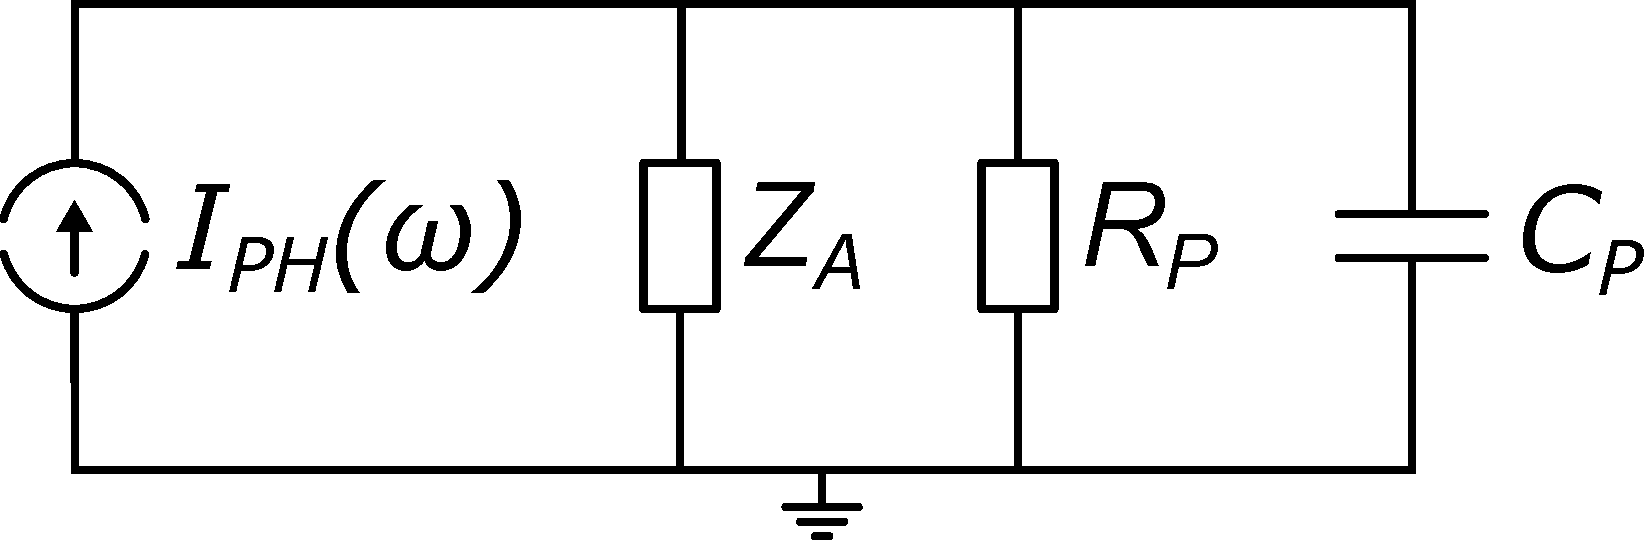
\includegraphics[width=0.7\textwidth]{figures/eq_circuit_PCA.pdf}
	\captionsetup{width=\textwidth}
	\caption{Equivalent circuit for a PCA, consisting of the antenna impedance $Z_A(\omega) = R_A + iB_A(\omega)$, the photoconductive resistance $R_P$ and the photoconductive capacitance $C_P$. The current source $I_{PH}(\omega)$ models the generated photocurrent.}
	\label{PCA_eq}
\end{figure}

Two roll-off factors decrease the emitted THz power at higher frequencies. RC roll-off reflects the influence of the PCAs capacitance and impedance. A PCAs equivalent circuit \cite{fernandezolveraInternationalSystemUnits2019,collinLimitationsTheveninNorton2003} is shown in figure~\ref{PCA_eq}. The current source $I_{PH}(\omega)$ models the radiating element of the antenna. In parallel to the radiating element sits the devices capacitance $C_P$ between the antennas electrodes. The resistance $R_P$ describes the photoconductivity $R_P^{-1} = G_P$ in parallel to the radiation resistance of the antenna $R_A$. Not all energy is radiated, some is stored in the susceptance $B_A(\omega)$. For simplicity, the radiation impedance is modelled as purely ohmic, leaving only $R_A$. Normally $R_{P} \gg R_A$, so the photoconductive resistance can be neglected.  With the made simplifications, the equivalent circuit represents a typical RC circuit in low-pass filter configuration. At higher frequencies, output power is expected to decrease. The current reaching the antenna is reduced by a factor $(1 + i2\pi \nu_{THz}\tau_{RC})^{-1}$, as can be shown by calculating the transfer function of the simplified equivalent circuit: 

\begin{equation}
    H = \frac{Z_{out}}{Z_{in}} = \frac{\frac{1}{i\omega C_P}}{R_A + \frac{1}{i\omega C_P}} = \frac{1}{1 + i\omega R_A C_P} = \frac{1}{1 + i 2\pi \nu_{THz} \tau_{RC}}.    
	\label{transferfunction}
\end{equation}

The factor by which output power will decrease is given by 

\begin{equation}
    \eta_{RC}(\nu_{Thz}) = \frac{1}{1+ (\nu_{THz}/\nu_{RC})^2} = |H|^2,  \qquad  \nu_{RC} = \frac{1}{2\pi\tau_{RC}} = \frac{1}{2\pi R_A C_P},
\end{equation}
where $\nu_{RC}$ is the RC 3 dB frequency.

Not all electron-hole pairs generated by photon absorption contribute to the photocurrent. A portion of charge carriers are trapped and recombine before reaching the electrodes. Due to recombination, the number of available charge carriers for photocurrent generation decreases exponentially over time. From eq. \eqref{eq8}, the average photocurrent over the transit time $\tau_{tr}$ can be calculated, yielding
\begin{align}
	I_{Ph}^{Id}(t) &= \frac{1}{\tau_{rec}} \int_{0}^{\infty} I^{Id}[1 + \cos(\omega_{THz}t + \phi)]e^{\frac{-t}{\tau_{rec}}}dt \notag \\
	I_{Ph}^{Id}(t) &=  I^{Id}\frac{\tau_{rec}}{\tau_{tr}}\left[
		1 + \frac{\sin(\omega_{Thz}t + \phi)}{\sqrt{1 + (\omega_{Thz} \tau_{rec})^2}}
	\right],
\end{align}
where $\tau_{rec}$ is the recombination time. Both the time dependent THZ part and the DC part of the photocurrent are damped due to the trapping of charge carriers by a factor $g = \tau_{rec} /\tau_{tr}$. The factor $g \ll 1$ is called the photoconductive gain. The THz part of the photocurrent is further decreased by the lifetime roll-off 
\begin{equation}
	\eta_{LT}(\omega_{THz}) = \frac{1}{1 + (\omega_{THz}\tau_{rec})^2}.
\end{equation}

In combination with the photoconductive gain $g$ this yields an intrinsic photoconductive roll-off
\begin{equation}
	\eta_{PC}(\omega_{THz}) = g^2\eta_{LT}(\omega_{THz}) = \frac{g^2}{1 + (\omega_{THz}\tau_{rec})^2}.
\end{equation}
Ultimately, the actual THz power emitted by a PCA is given by 

\begin{equation}
    P_{THz}(\omega) = \frac{1}{2}R_A(I_{Ph}^{Id})^2\eta_{ext}^2\eta_{PC}(\omega)\eta_{RC}(\omega).
    \label{eq_power}
\end{equation}

Considering the nonidealities is important for understanding high frequency limitations in THz-TDS setups. This work further evaluates how incorporating resistive elements into the antenna structure affects the mechanisms that limit THz performance. 


\subsection{Photoconductive Antennas for THz-TDS}

\begin{figure}[!]
    \centering
    \begin{minipage}{0.75\textwidth} 
        \centering
        \begin{subfigure}[t]{0.45\textwidth}
            \centering
            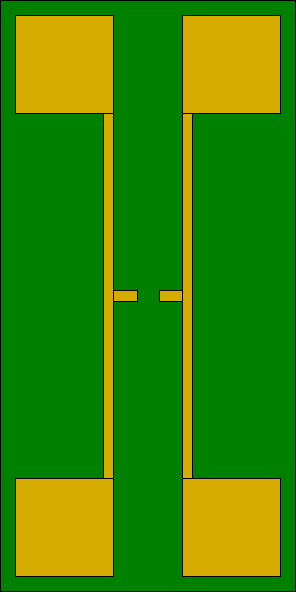
\includegraphics[height=0.32\textheight]{figures/typ_PCA_antenna.pdf}
            \caption{\centering}
            \label{fig:typPCAantenna}
        \end{subfigure}
        \hfill
        \begin{subfigure}[t]{0.45\textwidth}
            \centering
            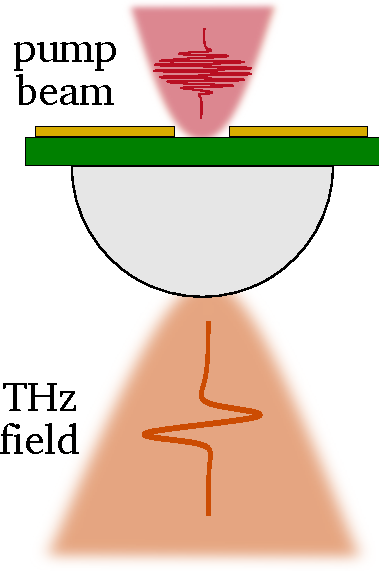
\includegraphics[height=0.32\textheight]{figures/typ_PCA_bias.pdf}
            \caption{\centering}
            \label{fig:typPCAbias}
        \end{subfigure}
        \caption{A typical PCA being used as a receiver in a pulsed system. (a) Typical PCA configuration depicting an H-Dipole antenna with a small active region in between the electrodes. (b) The charge carriers in the active region are optically excited by a femtosecond laser pulse. The device sits on top of a silicon lens. Incoming THz radiation is focused by the lens and biases the antenna.}
        \label{fig:typPCA}
    \end{minipage}
\end{figure}


% The testing of the fabricated devices in this work is limited to the detection of THz radiation. 

% THz antennas based on the photomixing technique usually consist of a small active region sitting in between the antenna's electrodes. For this thesis, the antennas will only be used as recipients for THz radiation. As discussed, PCAs need to be biased externally to emit or detect THz waves. When being used as receivers, the biasing in in PCA is provided by incident THz radiation focused onto the antenna's active region by a hyper-hemispherical silicon lens. A femtosecond laser beam is focused onto the active region as well, creating free electron-hole pairs (see figure~\ref{fig:typPCAbias}).
Figure \ref{fig:typPCA} shows a typical PCA alongside a schematic of its use as a detector in a THz-TDS system. A PCA generally exhibits a radiation resistance $R_A$ in the range of \num{20} - \num{200} \si{\Omega}. The detected THz power and bandwidth depend strongly on the antenna topology. Antenna types commonly used in CW operation, such as logarithmic periodic (log-periodic) antennas \cite{mendisTunableCWTHzSystem2004}, logarithmic spiral (log-spiral) antennas \cite{linRoomtemperatureContinuouswaveTerahertz2025}, or bow-tie antennas \cite{PDFBowtieWideband}, are not equally well suited for pulsed operation. Log-periodic and log-spiral antennas exhibit strong dispersion of THz pulses due to their long arms \cite{fernandezolveraDispersivePropertiesSelfcomplementary2017a}. Because a THz pulse spans multiple frequency components, different spectral parts of the pulse propagate differently within the antenna. Lower-frequency components with longer wavelengths travel more slowly, leading to temporal spreading and pulse distortion. Bow-tie antennas and complementary square spiral antennas \cite{HighPowerGeneration}, by contrast, exhibit lower dispersion and can enhance low-frequency components of the THz spectrum, thereby increasing the dynamic range (DNR).

The most commonly used PCAs in THz-TDS systems are H-Dipole antennas \cite{nandi1550nmDrivenErAs2018} (see Figure \ref{fig:typPCAantenna}) and slotline antennas \cite{kohlhaasPhotoconductiveTerahertzDetectors2019}. Both designs exhibit very low dispersion, which preserves the short duration and integrity of the generated THz pulses. Their  mostly non-dispersive broadband response, combined with a simple geometry, makes them the antennas of choice for many THz-TDS applications. Since this work focuses on improving PCA performance in pulsed operation, slotline antennas will not be discussed further. I-shaped resonant Dipole antennas are introduced as a point of comparison to H-Dipoles. I-shaped dipoles resonate at half the wavelength ($\lambda/2$) of the incident radiation and, like H-Dipoles and slotline antennas, are expected to show little dispersion. They are additionally predicted to provide enhanced sensitivity at lower THz frequencies \cite{nguyenPhotoconductiveDipoleAntennas2017}. I-shaped dipoles serve as a useful benchmark alongside H-Dipoles when evaluating the influence of NiCr modifications on antenna performance

The discussion above has outlined the working principles of PCAs under idealized
assumptions, where the generated photocurrent is directly coupled into free-space radiation. Some nonidealities have been described. Those however are mainly limited to the high-frequency performance of PCAs. This thesis addresses an additional limitation at the low-frequency end of the spectrum: resonances caused by the large metallic pads and antenna feeding structure. These resonances are typically not captured by the model derived above. Understanding these resonances is crucial since they limit the usable bandwidth of photoconductive antennas and motivate the central idea of this work: the introduction of resistive NiCr segments to damp low-frequency resonances. In the following section, the
origin and effects of these pad resonances are analyzed in detail.
